\documentclass{article}

\usepackage{ocencfd}
\usepackage{fancyvrb}
\usepackage{listings}

\title{NahamCon CTF 2022: Solutions} % Sets article title
\author{Arthur Verschaeve (hi@arthurverschaeve.be)}
\authorID{arthurvr}
\documentID{template}
\date{December 2022}

\begin{document}

\maketitle

\section{Warmups}
\subsection{Quirky}

The given text file looks like bytes with escape characters (\texttt{\textbackslash x}). The first few bytes are \texttt{89 50 4e 47}, which is the magic number of PNG images. I removed the escape characters and saved the bytes as a binary \texttt{.png} file, using the HxD freeware hex editor. The resulting image looks like a QR code.

\begin{center}
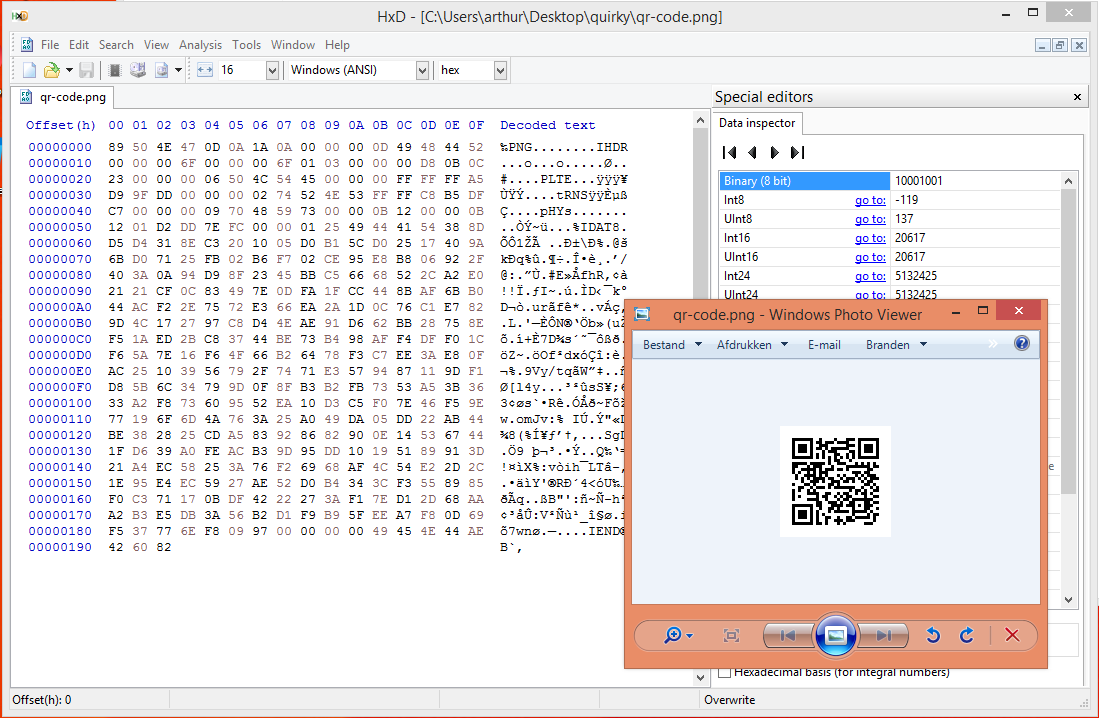
\includegraphics[width=16cm]{quirky/screenshot.png}
\end{center}
\noindent\newline There are a lot of utilities to read QR codes. I usually like zbar, but there are websites out there that can do it without an installation procedure too.

\noindent\newline Reading the code yields the correct flag: \texttt{flag\{b8e2a32f5ae629dcfb1ac210d1f0c032\}}

\subsection{Jurassic Park}

This is a classic \texttt{robots.txt} challenge. I opened the given website, found out there's not much interesting in the source code, so decided to check out its \texttt{robots.txt} file. This revealed a directory, which had an open directory listing with a \texttt{flag.txt} file. That file contains \texttt{flag\{c2145f65df7f5895822eb249e25028fa\}}.

\section{Cryptography}

\subsection{XORROX}

The operations inside the given script can easily be reversed, because the XOR-operation itself is reversible: Applying the same XOR operation with the original to encrypted data will decrypt it.  I did exactly that, copying part of the given loops, and pasting in the given values for \texttt{xorrox} and \texttt{enc}. After some simplifications (unused loop variables, for example), the script looks like this:

\lstinputlisting[language=Python, firstline=1, lastline=15]{XORROX/solution.py}

\noindent Executing this yields the following result:

\begin{Verbatim}[frame=single]
ag{21571dd4764a52121d94deea22214402}
\end{Verbatim}

\noindent The first characters, \texttt{"fl"}, are missing here because this reverse script doesn't perfectly imitate the start of the script, but that didn't matter, as we knew it was a \texttt{flag\{...\}}-formatted flag. \newline


\noindent
The flag is \texttt{flag\{21571dd4764a52121d94deea22214402\}}.

\subsection{Unimod}

The main (and only) operation in the given script is \texttt{chr((ord(c) + k) \% 0xFFFD)}, with \texttt{k} a randomly chosen integer between \texttt{0} and \texttt{0xFFFD}. This can be reversed using a subtraction (keeping the modulo), and for finding the value of $k$ a loop can be used. The following script finds the flag:

\lstinputlisting[language=python, firstline=1, lastline=15]{unimod/solution.py}


\noindent
The flag is \texttt{flag\{4e68d16a61bc2ea72d5f971344e84f11\}}.

\section{Hardware}
\subsection{Cereal}

I didn't know what the given file was at all. Some searching for the \texttt{.sal}-extension didn't yield much results either, but there was one forum question on something that seemed like hardware design tooling\footnote{https://discuss.saleae.com/t/utilities-for-sal-files/725}. I installed this \textit{SALAE - Logic 2} tool and indeed, it could open the file. The electrical signal contained in the what was apparently a capture file contained the flag:

\begin{center}
    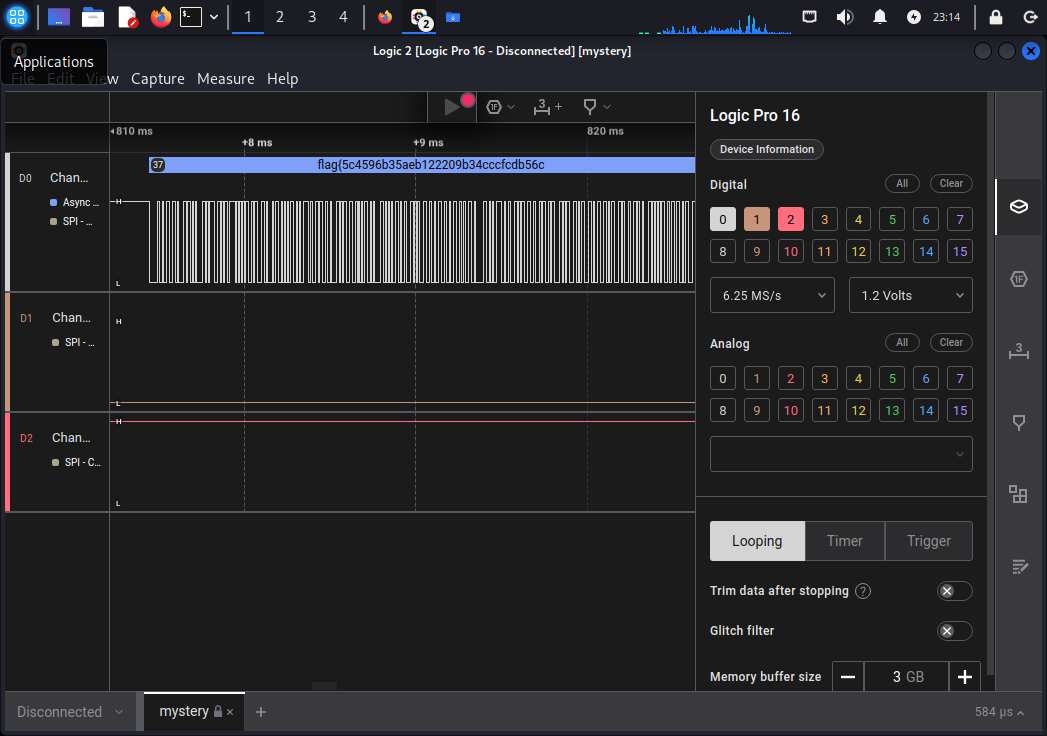
\includegraphics[width=16cm]{cereal/screenshot.png}
\end{center}

\noindent The flag is \texttt{flag\{5c4596b35aeb122209b34cccfcdb56c1\}}. 

\subsection{Dweeno}

I decided to not verify using the actual picture, and assume the sketch PDF was accurate. The \textit{4070} refers to XOR-gates, I found the datasheet for that component\footnote{https://pdf1.alldatasheet.com/datasheet-pdf/view/26894/TI/CD4070.html}. The following figure inside is all I really needed:

\begin{center}
    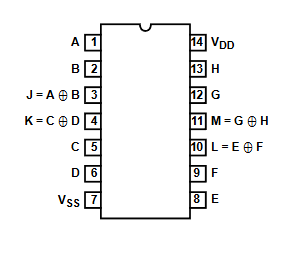
\includegraphics[width=5cm]{dweeno/datasheet-figure.png}
\end{center}

\noindent
Meaning the following relations follow from the given sketch (where $VX$ denotes the value on port $X$):

\begin{itemize}
    \item $V49 = V25 \oplus 0$
    \item $V23 = V47 \oplus 1$
    \item $V51 = V27 \oplus 1$
    \item $V29 = V53 \oplus 0$
\end{itemize}

\noindent
The first few lines of code within the code file indicate which ports are inputs and which are outputs. Continuing on the previously established relationships:

\begin{itemize}
    \item $out1 = in1 \oplus 0$
    \item $out2 = in2 \oplus 1$
    \item $out3 = in3 \oplus 0$
    \item $out4 = in4 \oplus 1$
\end{itemize}

\noindent
The program reads the bytes in the flag, and handles them 4 bits at a time through this electrical scheme. In other words, both the nibbles of the given bytes are XORed by $0b0101$. We can reverse this using a straightforward script:

\lstinputlisting[language=Python, firstline=1, lastline=15]{dweeno/solution.py}

\noindent
The flag is \texttt{flag\{a16b8027cf374b115f7c3e2f622d84bc\}}.
\section{Reverse Engineering}
\subsection{Babyrev}

After establishing that the given file is a standard executable, I opened it in the Ghidra reverse engineering tool. The main function is the following.

\noindent 
\begin{center}
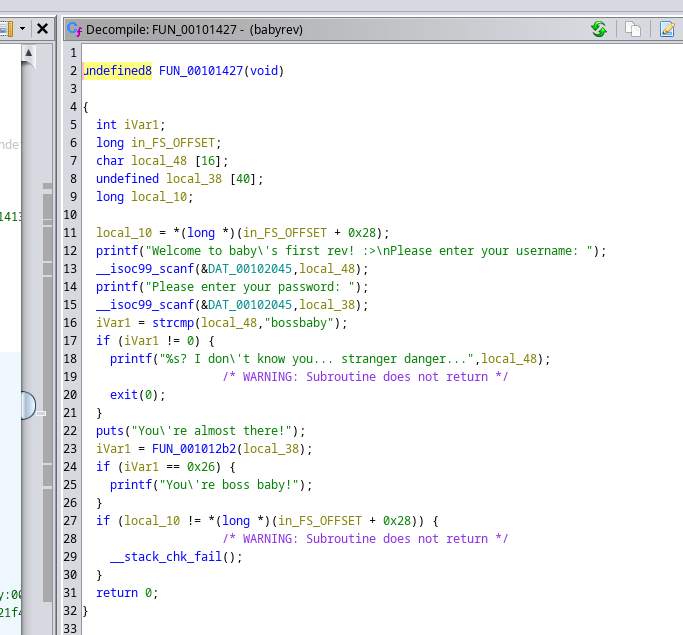
\includegraphics[width=13cm]{babyrev/screenshot1.png}
\end{center}

\noindent
It appears to check for a username first, which must be equal to \texttt{"bossbaby"}, and then do some kind of procedure to check the password. The procedure that checks the password must return \texttt{0x26}. I figured this password must be the flag, as those have always been of length 38. There does not seem to be anything dangerous in the file, so I executed it on my VM to confirm my first suspicions: 

\noindent 
\begin{center}
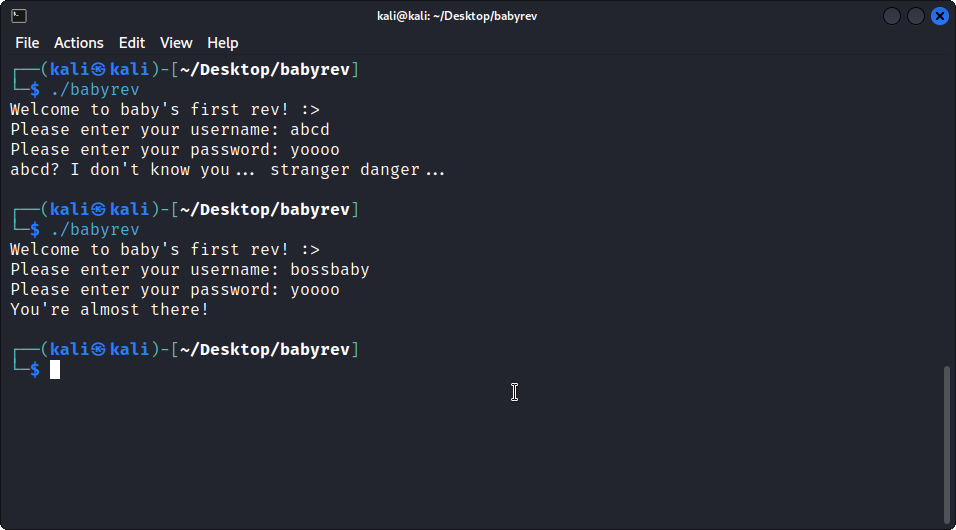
\includegraphics[width=16cm]{babyrev/screenshot2.png}
\end{center}

\noindent
Now, investigating the procedure that checks the password, the following lines seem essential. It is a length indeed, but the right length is only returned if some encoding of the password matches data hard coded at \texttt{\&DAT_00104020}. The alignment seems to be four bits, which was also confirmed with a manual look at the data there in memory.

\noindent 
\begin{center}
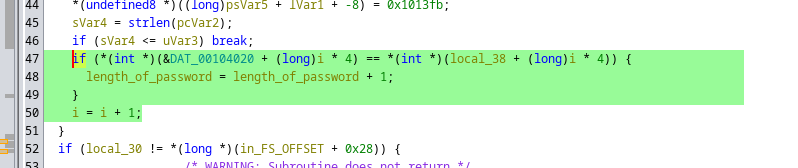
\includegraphics[width=16cm]{babyrev/screenshot3.png}
\end{center}

\noindent
The procedure which generates this encoding (\texttt{local_38}) is the following. It seems like a relatively simple calculation, which we can easily match in a Python script.

\noindent 
\begin{center}
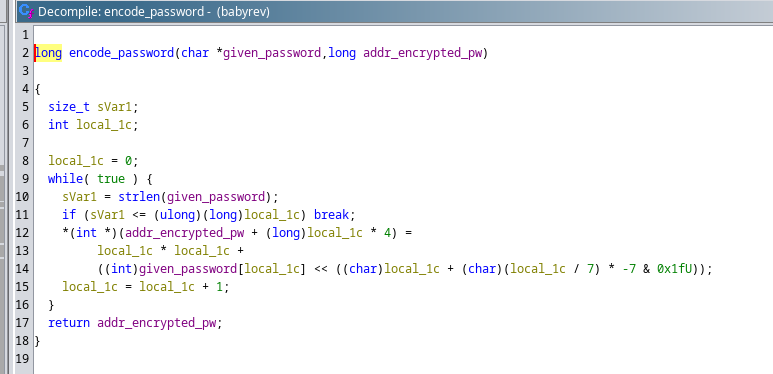
\includegraphics[width=16cm]{babyrev/screenshot4.png}
\end{center}

\noindent
Copying both the data we found and the calculation itself into Python, and creating a loop to try values of the flag byte-per-byte, we get the following. This script successfully generates the flag.

\lstinputlisting[language=Python, firstline=1, lastline=15]{babyrev/solution.py}

\noindent
The flag is \texttt{flag\{7bdeac39cca13a97782c04522aece87a\}}.

\section{Mobile}
\subsection{Mobilize (50 pts)}

I used \texttt{apktools} to decode the given APK file, and found the flag within \texttt{res/values/strings.xml}.

\begin{lstlisting}
...
<string name="exposed_dropdown_menu_content_description">Show dropdown menu</string>
<string name="fab_transformation_scrim_behavior">com.google.android.material.transformation.FabTransformationScrimBehavior</string>
<string name="fab_transformation_sheet_behavior">com.google.android.material.transformation.FabTransformationSheetBehavior</string>
<string name="flag">flag{e2e7fd4a43e93ea679d38561fa982682}</string>
<string name="hide_bottom_view_on_scroll_behavior">com.google.android.material.behavior.HideBottomViewOnScrollBehavior</string>
<string name="icon_content_description">Dialog Icon</string>
<string name="item_view_role_description">Tab</string>
...
\end{lstlisting}

\noindent
An alternative without the need to unpack the APK file could be using \texttt{strings} on the APK file:

\begin{lstlisting}
$ strings mobilize.apk | grep flag{
\end{lstlisting}

\noindent 
I verified, and this would have worked too. The flag is \texttt{flag\{e2e7fd4a43e93ea679d38561fa982682\}}.


\section{Keeber (OSINT)}
\subsection{Keeber 1}

I assumed I was gonna have to investigate \texttt{keebersecuritygroup.com}, it was the only website that showed up on Google that looked somewhat relevant. I used \textit{WHOIS} to find out who registered the domain. The flag showed up in the \texttt{Registrant Name} line:

\begin{Verbatim}[frame=single]
$ whois keebersecuritygroup.com
    Domain Name: KEEBERSECURITYGROUP.COM
    Registry Domain ID: 2689392646_DOMAIN_COM-VRSN
    Registrar WHOIS Server: whois.name.com
    Registrar URL: http://www.name.com
    Updated Date: 2022-04-15T01:52:49Z
...
    Registry Registrant ID: Not Available From Registry 
	Registrant Name: flag{ef67b2243b195eba43c7dc797b75d75b} Redacted 
	Registrant Organization:  
	Registrant Street: 8 Apple Lane  
	Registrant City: Standish 
	Registrant State/Province: ME 
	Registrant Postal Code: 04084 
	Registrant Country: US  
...
\end{Verbatim}

\noindent
The flag is \texttt{flag\{ef67b2243b195eba43c7dc797b75d75b\}}.

\subsection{Keeber 2}

The Wayback Machine is a great way to find ex-employees. In this case, the snapshot made on April 19 reveals one:

\noindent
\begin{center}
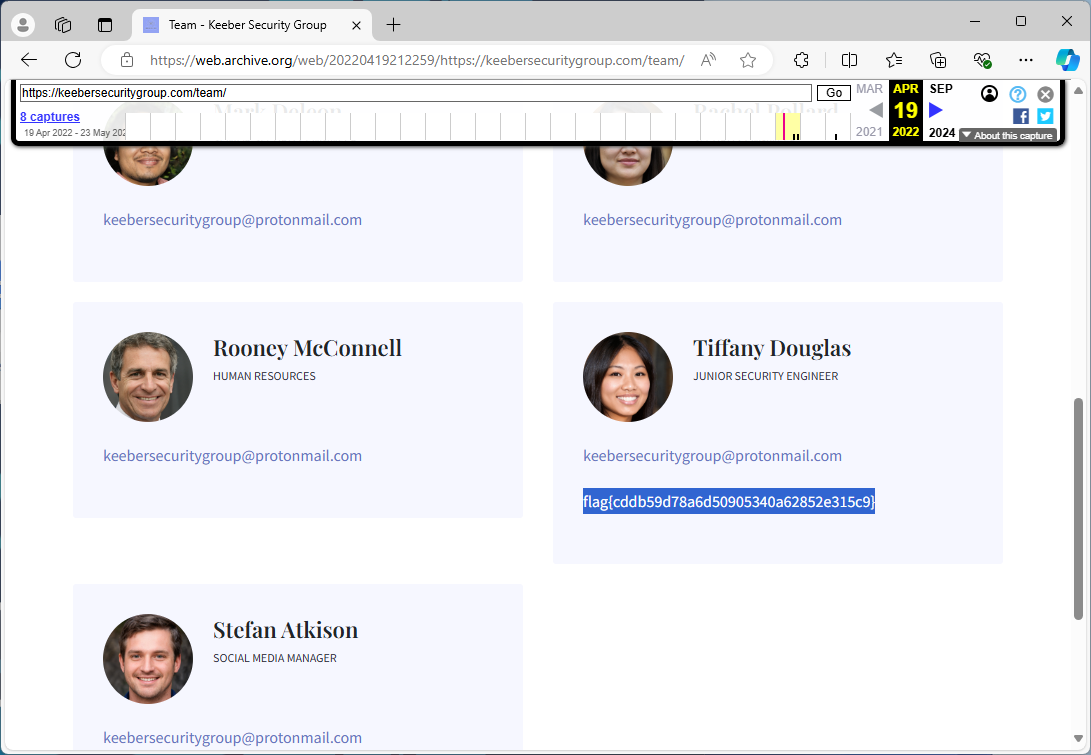
\includegraphics[width=16cm]{keeber2/wayback-machine.png}
\end{center}

\noindent
The flag is \texttt{flag\{cddb59d78a6d50905340a62852e315c9\}}.

\subsection{Keeber 3}

I figured the Git commit must be one on the \textit{@keebersecuritygroup} repositories on GitHub. The \textit{security-evaluation-workflow} repository has a \texttt{.gitignore} file containing a reference to \texttt{asana_secret.txt}, and the following commit specifically removing that file:

\noindent
\begin{center}
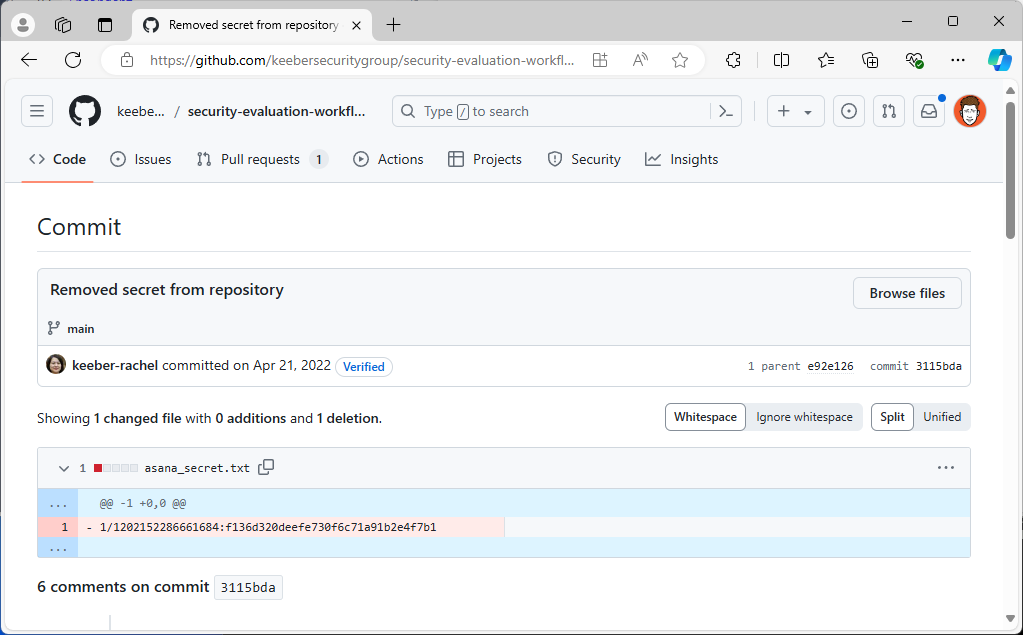
\includegraphics[width=16cm]{keeber3/screenshot1.png}
\end{center}

\noindent The \textit{Asana} platform has a documentation page on personal access tokens\footnote{https://developers.asana.com/docs/personal-access-token}, and this looks like one. The page contains an example \texttt{curl}-command to access the API, which I tried using the token.  The response contained the flag.

\noindent 
\begin{center}
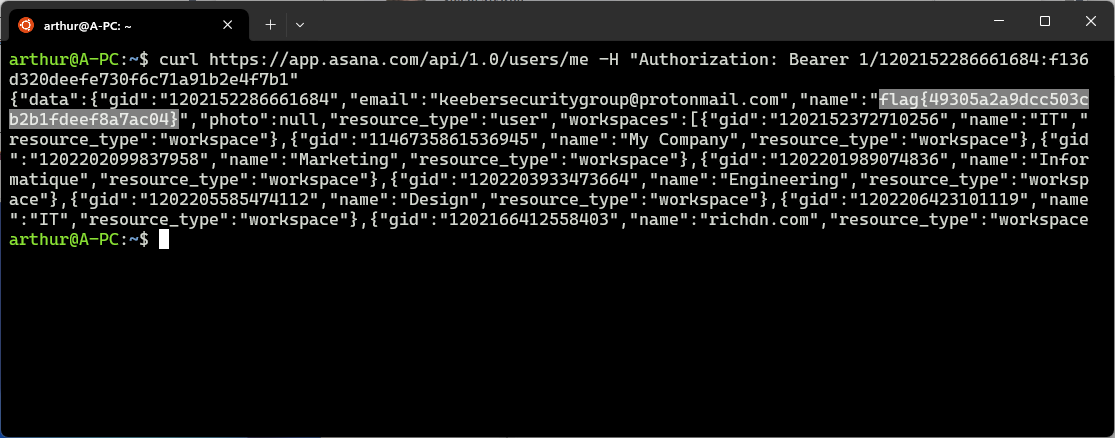
\includegraphics[width=16cm]{keeber3/screenshot2.png}
\end{center}
\noindent
The flag is \texttt{flag\{49305a2a9dcc503cb2b1fdeef8a7ac04\}}.

\subsection{Keeber 5}

The challenge text tells me the e-mail address I'm looking for is going to be in one of the commit histories. I could have accessed this on GitHub directly, but a search command seemed easier than reading everything myself. I did so using \texttt{git log | grep "flag"}, which immediately yielded the flag in the \textit{security-evaluation-workflow} repository. That's \texttt{flag\{2c90416c24a91a9e1eb18168697e8ff5\}}.

\section{Malware}
\subsection{USB Drive}

I first verified whether the given file was known malware. I used VirusTotal for this, which immediately yielded some results:

\noindent 
\begin{center}
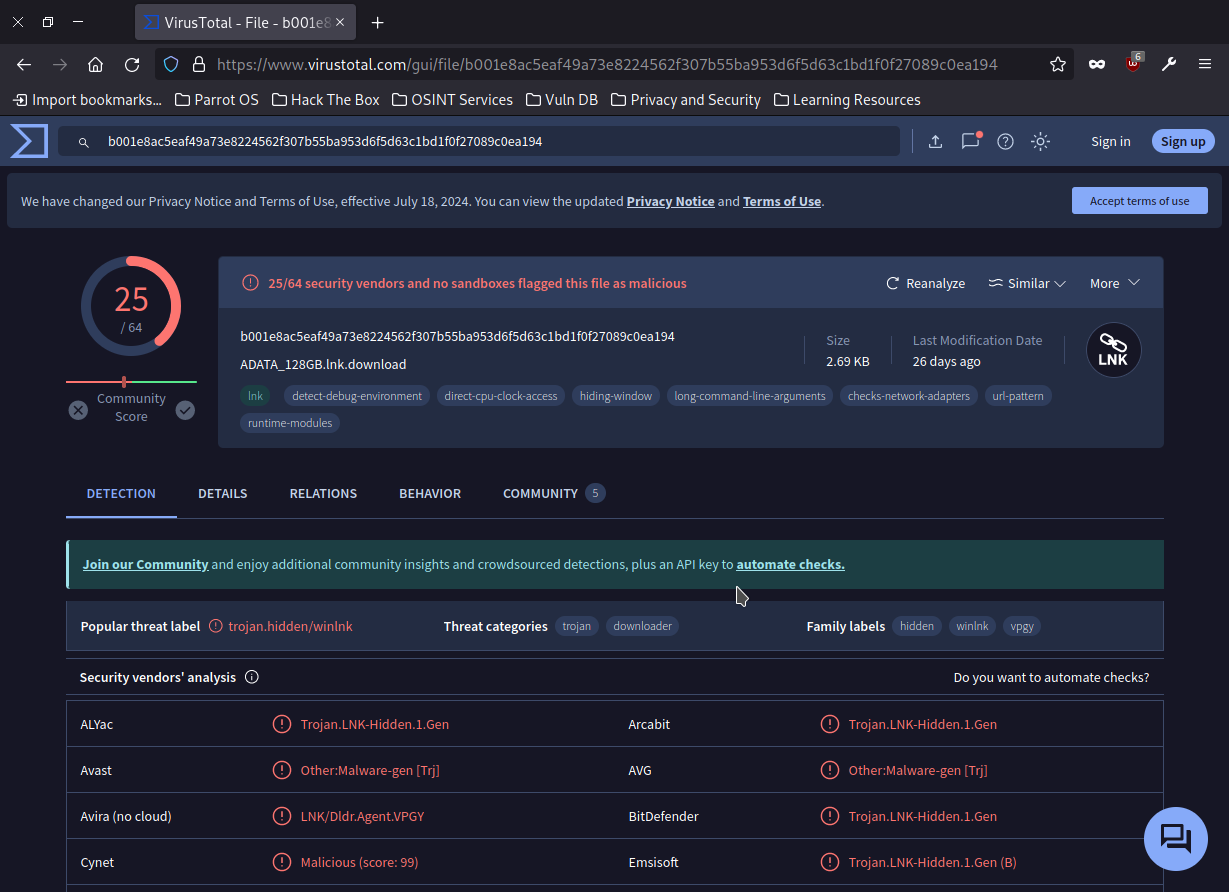
\includegraphics[width=16cm]{usb-drive/screenshot2.png}
\end{center}

\noindent
However, from these results, it was hard to check what exactly the file was doing, let alone find a flag. Using the \texttt{file} utility, I found out it's a Windows Shortcut file: this was already suggested by the \texttt{.lnk} extension.

\noindent 
\begin{center}
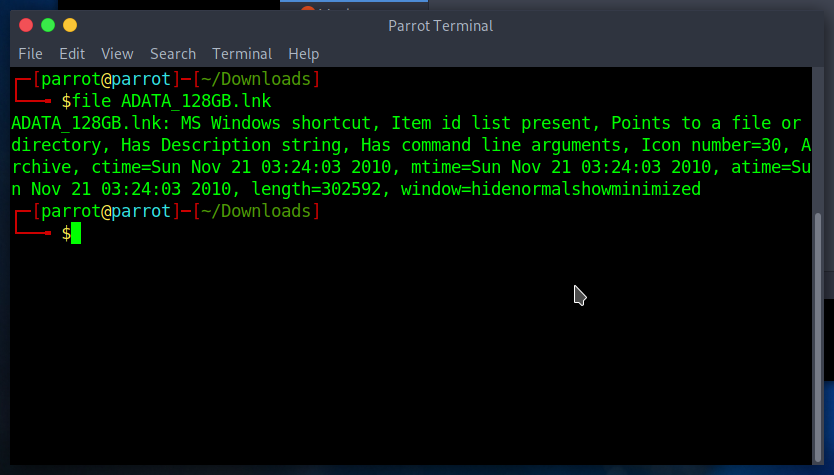
\includegraphics[width=16cm]{usb-drive/screenshot1.png}
\end{center}

\noindent
There exists a tool called \texttt{lnkinfo} which shows all the information in a \texttt{.lnk}-file. Calling it resulted in a lot of whitespace, which was probably an obfuscation attempt, but also a suspicious url: \texttt{https://tinyurl.com/a7ba6ma}.

\noindent 
\begin{center}
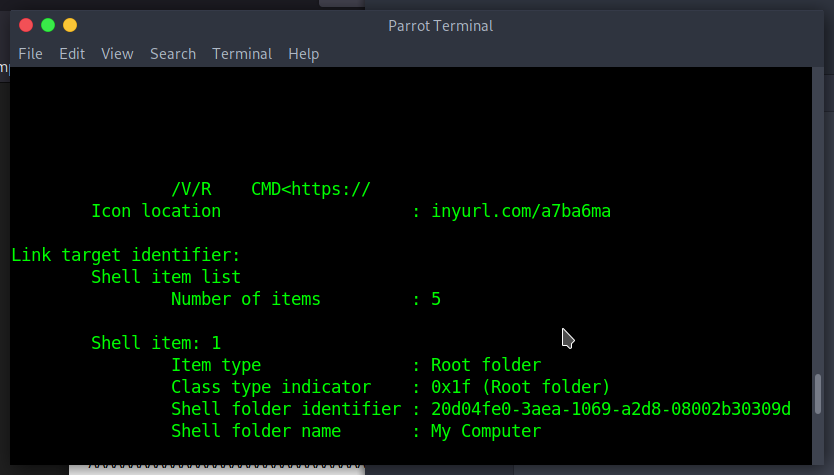
\includegraphics[width=16cm]{usb-drive/screenshot3.png}
\end{center}

\noindent
This url contained plain text, clearly some kind of encoding. My first guess was Base64 (which is popular in CTF challenges), but it turned out to be Base32. Decoding it resulted in an executable:

\noindent 
\begin{center}
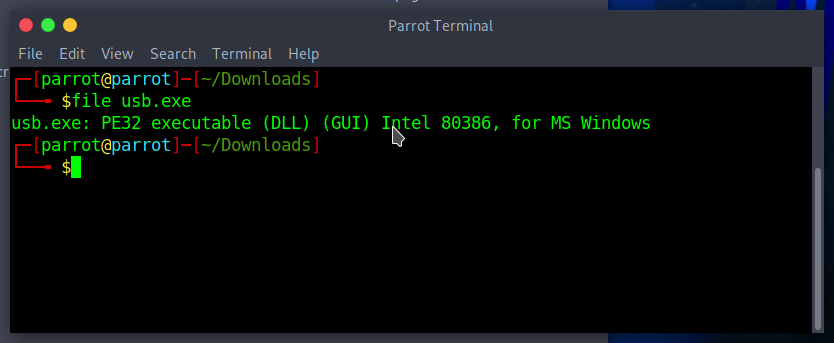
\includegraphics[width=16cm]{usb-drive/screenshot4.png}
\end{center}

\noindent
Which I dropped into the Ghidra reverse engineering tool, to get an insight into what the program does. It appears to print the flag: 

\noindent 
\begin{center}
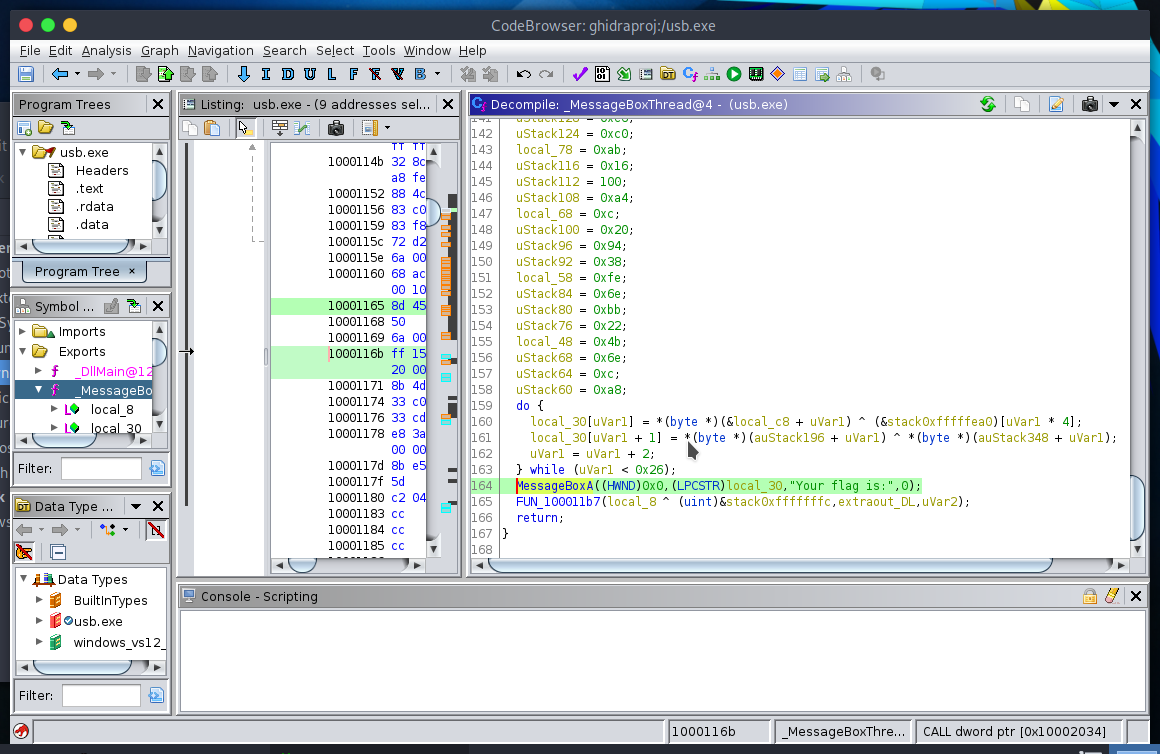
\includegraphics[width=16cm]{usb-drive/screenshot5.png}
\end{center}

\noindent
The loop with XOR operations on the preceding lines are probably meant to decode the flag first. I could write code to simulate those operations, which would take some time but would definitely work. Another option would be to execute the script: if it really only prints something, that is supposed to be safe. I went with a third option: I used emulation, specifically speakeasy\footnote{https://github.com/mandiant/speakeasy}.

\noindent 
\begin{center}
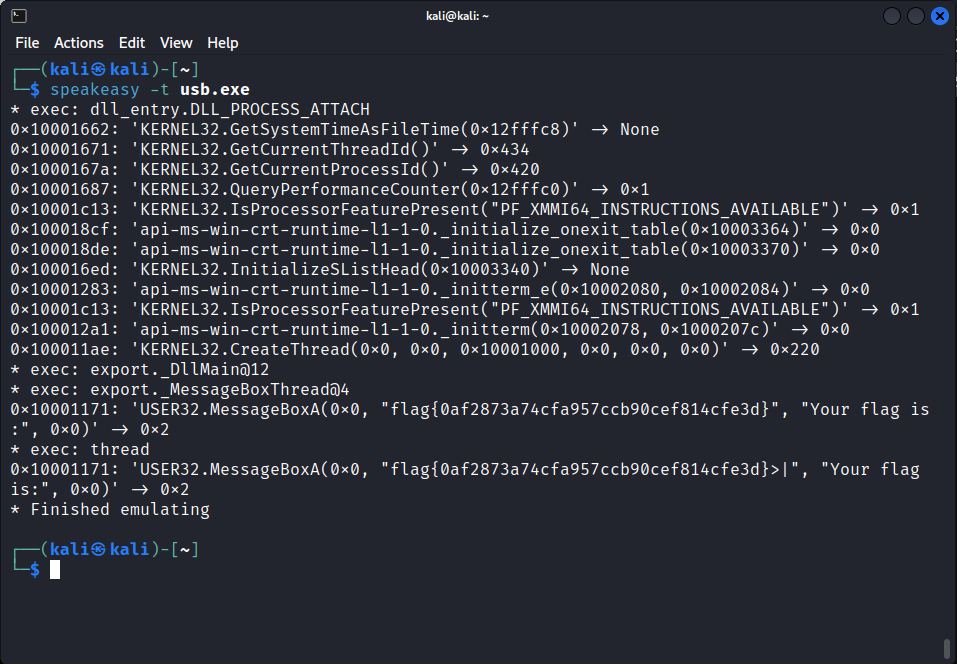
\includegraphics[width=16cm]{usb-drive/screenshot6.png}
\end{center}

\noindent
The flag is \texttt{flag\{0af2873a74cfa957ccb90cef814cfe3d\}}.

\end{document}
